\documentclass[a4paper, 11pt]{book}
\usepackage[utf8]{inputenc}
\usepackage{mathtools, amssymb, graphicx, amsmath, epstopdf}

\title{Notes on Information Theory}
\author{Cristian Di Pietrantonio, Michele Laurenti, Lorenzo Madeddu}

%ambients
\newtheorem{thm}{Theorem}
\newtheorem{obs}{Observation}

%math symbols
\newcommand{\sfrac}{\frac}
\newcommand{\Tau}{\mathrm{T}}                         %Capital Tau
\newcommand{\ifrac}[2]{{#1}/{#2}}                     %Inline fraction
\newcommand{\str}[1]{\underline{#1}}                  %String 
\newcommand{\msgset}{\mathcal{M}}                     %the set of all messages
\newcommand{\hball}[2]{B_H(\str{#1}, #2)}             %the Hamming ball
\newcommand{\hdist}[2]{d_H(\str{#1}, \str{#2})}       %Hamming distance
\newcommand{\hweight}[1]{w_H(\str{#1})}               %Hamming weight

\begin{document}
	\maketitle
	
	\chapter{Introduction}
	\section{Lesson 1}

Information Theory is born from one man, Cloude Shannon (1926 - 2001); it has to do with probability, algebra, coding theory, ergodic theory and appears in daily life. In communication you want to be understood, but you also want to avoid redundancy and words tend to be lengthy; there is a conflict of interest. Why some words are short and others are long? Short words encode common abstract pictures whereas long words must carry the whole information not available in common knowledge [nessuna fonte].\\

Suggested readings: 
\begin{itemize}
	\item Tom Cover, Joy Thomas, Information Theory, Wiley;
	\item IT: cooling theorems for discrete memoryless systems, Korner;
	\item IT, Robert Ash.
\end{itemize}

	
\section{Lesson 2}
Define $\msgset$ as the finite set of all messages over an alphabet $\Sigma$. A message $m$ is an element of $\msgset$. Hartley, who introduced this concept before Shannon, stated that the maximum amount of information is equal to $\log_2 |\msgset|$, since one can identify elements of $\msgset$ with binary strings of length $\log_2 |\msgset|$. Formally $$\msgset \sim \{0, 1\}^{\lc\log_2 |\msgset|\rc} $$ and $$ m \sim \Delta \in \{0, 1\}^{\lc\log_2 |\msgset|\rc}.$$

One can think of $\Delta$ as a sequence of $\log_2 |\msgset|$ binary questions that identify an element in $\msgset$; a single unit of information is a $0$ or $1$ (Binary Information Theory). In the \emph{20 question game}, where you need to minimize the number of questions to guess what a person thinks, is given a probability distribution $P$ over $\msgset$ s.t. $P(m) \geq 0,\ \forall m \in \msgset$ and $\sum_{m \in \msgset} P(m) = 1$. The questions can be designed to make the game as short as possible if $P$ is known.

Must be noted that $|\underline{x}| = i \Leftrightarrow \underline{x} \in \{0, 1\}^{i}$. The number of questions asked on average must be minimized. Let $f: \msgset \rightarrow \{0, 1\}^*$, in other words a mapping from the message set to the sequences of answers to find the message then we want to minimize 
\begin{equation} \label{eq:problen}
\sum_{m \in \msgset} P(m) |f(m)|.
\end{equation} 
This equation is tied only to the probability distribution, not to the set or the questions. If $P$ is uniform then \ref{eq:problen} is equal to $\lc\log_2 |\msgset|\rc$. The function $f$ is called \textbf{code}. The code is not always invertible.

Communication happens at a distance, otherwise it would be trivial. There is some device that makes communication possible; the channel is not perfect. The noise no it is random, modelled through a probability distribution. The information source is not predictable either and will have itsoen probability distribution too ['nche senso, di errore o tempo di trasmissione?]. Encoding and decoding must be optimized to make communications short to reduce ``lost'', and to reliably transmit, i.e. the receiver is reasonably sure that it gets what was sent. The two aspects are in contrast, you need and optimal trade-off. Usually partners in communication are separated in space and communication takes place in time. Sometimes in computer science the opposite thing happens: communication is storing information in space to retrieve it later in time. Sometimes you want to shorten the communication time, sometimes the space communication takes. The model is the same. Entropy comes from thermodinamics, introduced by Boltzmann.
	%October 2016, the 4th
\section{Lesson 3 - Hamming Space}

A space is a set that has structure. Consider the set of all binary strings $\{0, 1\}^*$; we can define a space with the distance metric. The \textbf{distance} is defined as a function $d: X \times X \rightarrow \mathbb{R}^+_0$. A metric has the following properties:
\begin{enumerate}
	\item \begin{enumerate}
		\item $d(x, y) \geq 0,\ \forall (x, y) \in X \times X$
		\item $d(x, y) = 0 \Leftrightarrow x = y$
	\end{enumerate}
	\item $d(x, y) = d(y, x), \forall (x, y) \in X \times X$
	\item $d(x, y) \leq d(x, z) + d(z, y)$
\end{enumerate}

What is the Hamming metric? Consider $\str{x}, \str{y}  \in \{0, 1\}^n$. Then the Hamming distance is defined as
\begin{equation}
	\hdist{x}{y} = |\{i\ |\ x_i \not= y_i\}|
\end{equation}

Why is it a metric? Consider $\str{x}$, $\str{y}$, $\str{z} \in \{0,1\}^n$. Then, with $D = \{i\ |\ x_i \not= y_i\}$ is true that 
\begin{center}
	\begin{math}i \in D \Rightarrow x_i \not=y_i \Rightarrow \neg (z_i = x_i \wedge z_i = y_i) \Rightarrow d_H(x_i, y_i) \leq d_H(z_i, x_i) + d_H(z_i, y_i).
	\end{math}
\end{center}

By the additive property we can write $$d_H(x, y) = \sum_{i = 1}^n d_H(x_i, y_i).$$ Summing up gives the triangle inequality.

If a string $\str{x}$ has been changed $r$ times to become $\str{y}$ then $d_H(\str{x}, \str{y}) \leq r$. Define a \textbf{Hamming ball} of radius $r$ around $\str{x}$ as 
$$B_H= \hball{x}{r} = \{\str{y}\ |\ \hdist{x}{y} \leq r\}.$$
Obviously $r$ needn't to be an integer (use the \emph{floor} function). Here are some properties of Hamming balls:
\begin{itemize}
	\item if one subtracts $\hball{x}{r}$ to $\{0, 1\}^n$ then the result is also an Hamming ball;
	\item $\{0, 1\}^n = \hball{x}{n},\ \forall \str{x} \in \{0, 1\}^n$, but if $r < n$ then the center is unique;
\end{itemize}

What we can say about $\hball{x}{r}$? For simplicity sake, consider $\hball{0}{r}$. Then the following holds:
\begin{equation}\label{eq:volume}
	|\hball{0}{r}| = \sum_{i = 0}^{\lfloor r \rfloor} \binom{n}{i}
\end{equation}

That is the number of ways in which we can flip to 1 the bits. From this follows that $\hdist{0}{y} + \hdist{1}{y} = n$.

We define the Hamming weight as $\hweight{x} = \hdist{0}{x}$. The following holds:
$$\str{y} \in \hball{0}{r} \Rightarrow \hweight{y} > r \Rightarrow \hdist{y}{1} < n - r \leq n -r - 1.$$

So it is true that

$$\overline{\hball{0}{n}} = \hball{1}{r'} = \hball{1}{n - r - 1}.$$

In other words the Hamming space can be partitioned into two Hamming balls. If $n$ is odd an Hamming space can be partitioned in the following way: $$\{0, 1\}^n = \hball{0}{\lfloor \dfrac{n}{2}\rfloor } \cup \hball{1}{\lfloor \dfrac{n}{2}\rfloor}$$
The Hamming space cannot be partitioned into three balls. In how many balls can $\{0, 1\}^n$ be partitioned? It cannot partitioned be partititoned into $s$ balls with $3 \leq s \leq n + 1$.

\subsection{The volume of a Hamming ball}
We have seen that the volume of a generic Hamming ball is described by equation \ref{eq:volume}. We can use the Pascal triangle to get a feeling about the order of magnitude of the Hamming ball. Consider the $n$th row in the triangle; since it is symmetric, if we split the row in half the sum of the terms of the first part is equal to the sum of the terms of the second part of the row. The volume of the greatest ball is $|\hball{0}{n}| = 2^n$; instead, the volume of the ball with radius $n/2$ (in the triangle's point of split) is $\ifrac{2^n}{2} = 2^n2^{-1} = 2^{n-1}$. So, if $r \geq \ifrac{n}{2}$ then $2^{n-1} \leq |\hball{0}{r}| \leq 2^n$. Can we bound the volume for $r < \ifrac{n}{2}$?

First we introduce the notion of \textbf{entropy}, a function $h: [0, 1] \rightarrow [0, 1]$ defined as follows:
\begin{center}
	$h(t) = t\log_2(\dfrac{1}{t}) + (1 - t)\log_2\left(\dfrac{1}{1-t}\right)$
\end{center}

The plot of $h$ looks like this:
\begin{figure}[h]
	\centering
	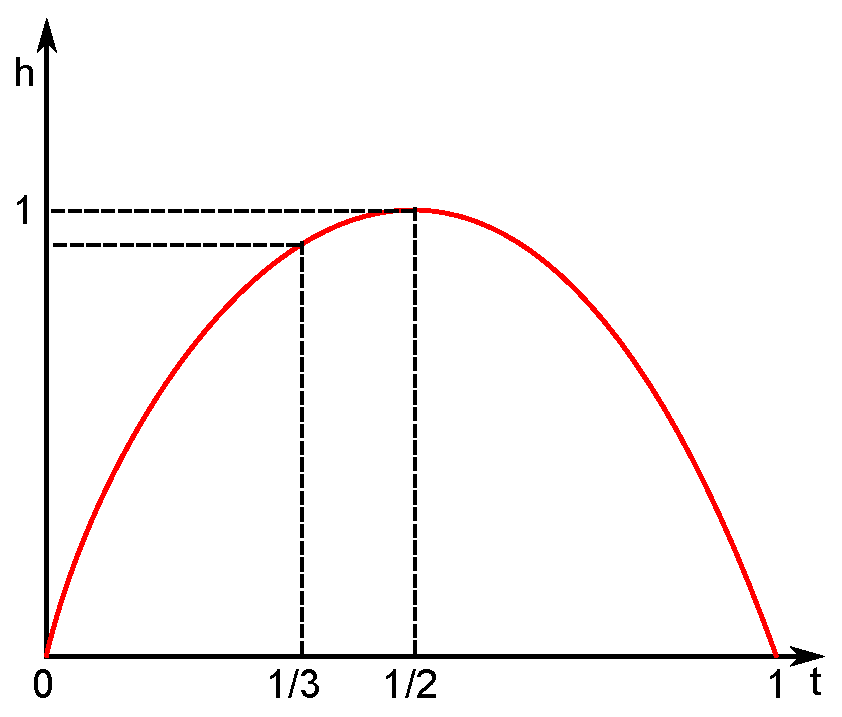
\includegraphics[width=210px]{pictures/ch01-i00.eps}
	\caption{The entropy function.}
\end{figure}

This function is not defined for the values $0$ and $1$ but we have limits defined on these points, and they are both $0$. So we artificially set $h(0) = 0$ and $h(1) = 0$. It is better to think about it as probability distribution $(t, 1 - t)$ and entropy is a number attached to it. Entropy measures symmetry and with $t = \ifrac{1}{2}$ we have maximum chaos (the future outcomes are equally likely). % October 2016, 4th
	\section{Lesson 4}

\begin{thm}
	The upper bound on the volume of a Hamming ball, if $ r \leq \ifrac{n}{2}$, is
	$$|\hball{0}{r}| \leq 2^{nh\left(\sfrac{r}{n}\right)}$$
\end{thm}

In order to prove this theorem an analogy is introduced. Suppose there is a box with a number of chickens in it. We want to count those animals without withdrawing all of them out of the box. What can be done is to take the lightest one and measure its weight $w$; then also the weight $W$ of the box is measured. The number of the total chickens in the box can't be greater than $\ifrac{w}{W}$.\\

\noindent\textbf{Proof.} In this proof we will use a similar technique. Consider $\{0, 1\}^n$. We ``sparkle'' a substance on the strings in the set; this substance looks like probability, but it doesn't matter. Define the weight of $1$ and $0$ as 
$$P(1) = \dfrac{r}{n},\ P(0) = 1 - P(1).$$

Notice that is not an uniform distribution. Define the weight of a string as
$$P^n(\str{x}) = \prod_{i = 1}^n P(x_i).$$

If $A \subseteq \{0, 1\}^n$ then the weight of the set $A$ is $$P^n(A) = \sum_{\str{x} \in A} P^n(\str{x}).$$

$P^n(\{0, 1\}^n)$ is the total weight of the substance sparkled on the strings and it is the probability distribution of binomial. For this reason one can claim that
$$1 = P^n(\{0, 1\}^n) \geq P^n(\hball{0}{r}) = \sum_{\str{x} \in \hball{0}{r}} P^n(\str{x})$$

at this point we ``take out the lightest chicken'' and write
$$\sum_{\str{x} \in \hball{0}{r}} P^n(\str{x}) \geq |\hball{0}{r}| \cdot \min_{\str{x} \in \hball{0}{r}}P^n(\str{x})$$

Which are the lightest chickens? Because we assume $r \leq \ifrac{n}{2}$ then
$$r \leq \dfrac{n}{2} \Rightarrow P(1) = \dfrac{r}{n} \leq \dfrac{1}{2} \Rightarrow P(1) \leq P(0).$$
It follows that the the lightest strings are the ones on the border of the ball, with $r$ $1$'s. We now compute their weight.

\[\min_{\str{x} \in \hball{0}{r}}P^n(\str{x}) = [P(1)]^r\cdot[P(0)]^{n-r} = \] 
\[ = \left(\dfrac{r}{n}\right)^r \left(1 - \dfrac{r}{n}\right)^{n-r} = \]  \[ = \left(\dfrac{r}{n}\right)^{n\sfrac{r}{n}} \left(1 - \dfrac{r}{n}\right)^{n\left(1 - \sfrac{r}{n}\right)} =\]
\[ = [\left(\dfrac{r}{n}\right)^{\sfrac{r}{n}} \left(1 - \dfrac{r}{n}\right)^{\left(1 - \sfrac{r}{n}\right)}]^n =\] 
\[ =2^{n\log_2[\left(\sfrac{r}{n}\right)^{\sfrac{r}{n}}  \left(1 - \sfrac{r}{n}\right)^{\left(1 - \sfrac{r}{n}\right)}]} = \]
\[ =2^{n[\sfrac{r}{n}\log_2\sfrac{r}{n} + \left(1 - \sfrac{r}{n}\right)\log_2\left(1 - \sfrac{r}{n}\right)]} = 2^{-nh\left(\sfrac{r}{n}\right)}\]

So we have 

\[1 \geq |\hball{0}{r}| \dfrac{1}{2^{nh(\sfrac{r}{n})}} \Rightarrow |\hball{0}{r}| \leq 2^{nh\left(\sfrac{r}{n}\right)}\] 
\hfill$\Box$


\begin{thm}
	The lower bound on the volume of a Hamming ball, if $ r \leq \ifrac{n}{2}$, is
	$$|\hball{0}{r}| \geq \dfrac{1}{n+1}2^{nh(\sfrac{r}{n})}$$
\end{thm}

\noindent\textbf{Proof.} $$P(1) = \dfrac{r}{n},\ P(0) = 1 - P(1),\ P^n(\{0, 1\}^n) = 1.$$
Consider the set of all strings of length $n$ and partition it in the following way.
$$\Tau_q^n = \{\str{x}\ |\ \hweight{x} = q\},$$
obtaining $n +1$ classes. 
We know that $|\Tau_q^n| = \binom{n}{q}$; we are not interested in how many strings are in that set, but what is the total weight; we want to prove $$ |T_r| \geq \dfrac{1}{n+1}2^{nh\left(\sfrac{r}{n}\right)}.$$ There is not symmetry in the weight of the partitions so there is a weight $r$ so that
$$ \dfrac{P^n(\Tau_q)}{P^n(\Tau_r)} \leq 1,\ \forall q$$
In the formula above there are binomials we want to bound.

\begin{obs}
	$$\dfrac{k!}{l!} \leq k^{k-l}.$$
\end{obs}

\noindent\textbf{Proof}. We are going to prove this observation in two steps.
\begin{itemize}
	\item $k \geq l$. 
		$$\dfrac{k!}{l!} = \dfrac{k(k-1) \cdots l(l -1) \cdots 1}{l(l -1) \cdots 1} \leq k^{k-l}.$$
		
	\item $k < l$.
		$$\dfrac{k!}{l!} = \dfrac{k(k-1) \cdots 1}{l(l -1) \cdots k(k-1) \cdots 1} \leq \left(\dfrac{1}{k+1}\right)^{l-k} < \left(\dfrac{1}{k}\right)^{l-k} = k^{k-l}.$$
\end{itemize}
\hfill$\Box$

% Lesson5
Define $p = \ifrac{r}{n}$  so that we have a distribution $P(p, 1-p)$ that picks a set and concentrate the weight (probability) on it. We observe that the probability of each string in a class depends only on the number of $1$'s in it. So we can write

\[\dfrac{P^n(\Tau_q)}{P^n(\Tau_r)} = \dfrac{p^q(1-p)^{n-q}|\Tau_q|}{p^r(1-p)^{n-r}|\Tau_q|} = p^{q-r}(1-p)^{r-q} \dfrac{\frac{n!}{q!(n-q)!}}{\frac{n!}{r!(n-r)!}} = \]
\[ = p^{q-r}(1-p)^{r-q}\dfrac{r!}{q!}\dfrac{(n-r)!}{(n-q)!} \leq p^{q-r}(1-p)^{r-q}r^{r-q}(n-r)^{q-r} = \]

considering that $r = np$ it follows that

\[p^{q-r}(1-p)^{r-q} (np)^{r-q}[n(1-p)]^{q-r}=p^{q-r}(1-p)^{r-q}n^{r-q+q-r}p^{r-q}(1-p)^{q-r} = \]

\[ = p^{q-r + r-q}(1-p)^{r-q+q-r} = 1.\]

So we can write

\[1 = P^n(\{0,1\}^n) = P^n\left(\bigcup_{q=0}^nT_q\right) = \sum_{q=0}^nP^n(T_q)\leq(n+1) \max_qP^n(T_q) = \]

\[=(n+1)P^n(T_r) = (n + 1)|T_r|2^{-nh\sfrac{r}{n}}\]
	
From the previous result we know $|T_r| \geq \dfrac{1}{n+1}2^{nh(\sfrac{r}{n})}$ and $T_r \subseteq \hball{0}{r}$ so it follows that $|T_r| \leq |\hball{0}{r}|$. \hfill $\Box$

So this proof is important because of two reasons:

\begin{enumerate}
	\item something related to entropy. [LISTEN THE REGISTRATION];
	\item Cardinality of the Hamming ball comes up in error correction (a string that has been haltered at most $r$ times is in a certain radius from the original string).
\end{enumerate}
	\section{Lesson 13/10/2016}

Let $\xset$ be the (usual) finite set that is an alphabet; the interest lies in sequences of elements of $\xset$, called \emph{strings} or \emph{words}. So $\xset^n, n \in \mathbb{N}$, is a set of words. $\xset^n$ can be partitioned by putting together those sequences that can be transformed one into the other by permutation, i. e. sequences that have the same number of occurrences of elements in the alphabet.

Let $a \in \xset$ and $\str{x} \in \xset^n$. We define the frequency of an alphabet symbol $a$ in a string $\str{x}$ in the following way:  
\begin{equation}
N(a | \str{x}) = |\{i\ |\ x_i = a\}|,
\end{equation}

where $\str{x} = x_1x_2\ldots x_n$. One can think about ``normalized'' relative frequencies of symbols $$\dfrac{1}{n} N(a|\str{x}).$$

Moreover the following holds:

$$\sum_{a \in \xset} N(a|\str{x}) = n \Rightarrow \sum_{a\in \xset} \dfrac{1}{n}N(a|\str{x}) = 1$$

so from a string $\str{x}$ one can obtain a probability distribution over $\xset$. We define
\begin{equation}
	P_{\str{x}} = \left\{ \dfrac{N(a|\str{x})}{n}\ |\ a \in \xset \right\}
\end{equation}
to be the \emph{type} of $\str{x}$. There are just that many distributions for a number $n$; now fix a distribution $P|\xset$. $\exists \str{x} \in \xset^n$ such that  $P_{\str{x}} = P$? Yes, if and only if
$$P(a) = \dfrac{N(a | \str{x})}{n},\ \forall a \in \xset.$$ Consider a product measure over $\xset$; strings in the same partition have also the same ``length'' or measure. Now, given $\xset$ and $n$, how many distributions $P|\xset$ are types in $\xset^n$? A rough upper bound is $(n + 1)^{|\xset|}$. The last value is redundant, since the values sum up to $1$. So we could do better with $(n + 1)^{|\xset| - 1}.$ We can partition $\xset^n$ into sets of strings of the same type, $\Tau_p$, with $P|\xset$. $$\Tau_p = \Tau_p^n = \{\str{x}\ |\ P_{\str{x}} = P\}.$$

\begin{thm} \label{thms:taupcard}
	If $\Tau_p \not= \emptyset$ then $$\dfrac{1}{(n+1)^{|\xset| -1}}2^{nH(p)}\leq |\Tau_p| \leq 2^{nH(p)}$$
\end{thm}

\noindent\textbf{Proof.} In order to prove the above theorem, we first define the product distribution $P|\xset \rightarrow P^n|\xset^n$ as 
\begin{equation}
	P^n(\str{x}) = \prod_{i = 1}^nP(x_i).
\end{equation}

We can define it additively on subsets of $\xset^n$.
\[
1 = P^n(\xset^n) \geq P^n(\Tau_p^n)
\]

We also introduce the \emph{generalized entropy} $H(P)$, defined as $$H(P) = -\sum_{a \in \xset} P(a)\log_2P(a).$$
Now,

\[
\forall \str{x} \in \Tau_p^n P^n(\str{x}) = \prod_{a \in \xset}P(a)^n = nP(a)
\]
notice that this is independent from $\xset$. So we have

\[ 
= \prod_{a \in \xset} 2^{nP(a)\log_2P(a)} = 2^{n\left[\sum_{a \in \xset} P(a)\log_2P(a)\right]} = 2^{-nH(p)}
\]

So,

\[1 = P^n(\xset^n) \geq P^n(\Tau^n_p) = |\Tau_p^n|2^{-nH(p)} \] $\hfill\Box$

The lower bound proof is a straightforward generalization of what has been don in the binary case.

\section{IDK what he's talking about yet (always 13/10)}
Entropy is greatest when the distribution is uniform. Now, to the lower bound.
\[
1 = \sum_{P\ |\ \Tau_p^n \not= \emptyset}P^n(\Tau_p^n) \leq (n+1)^{|\xset|-1} \max_{Q|\xset}P^n(\Tau_q^n)
\]

\begin{obs}
If $\Tau_p \not= \emptyset$ then $$\dfrac{P^n(\Tau^n_q)}{P^n(\Tau^n_p)} \leq 1$$
\end{obs}

If a distribution is a type, it maximizes its (product) value on the strings of that type. We can suppose without loss of generality (w.l.o.g) that $\Tau^n_q \not= \emptyset$.
\[
P^n(\Tau_q^n) = \prod_{a \in \xset} P(a)^{nQ(a)}|\Tau_q^n| \Rightarrow \dfrac{P^n(\Tau_q^n)}{P^n(\Tau_p^n)} = \dfrac{|\Tau_q|^n\prod_{a \in \xset}[P(a)]^{nQ(a)}}{|\Tau_p|^n\prod_{a \in \xset}[P(a)]^{nP(a)}} =
\]

\[
 = \dfrac{\dfrac{n!}{\prod_{a\in\xset}[nQ(a)]!}\prod_{a\in\xset}[P(a)]^{nQ(a)}}
 {\dfrac{n!}{\prod_{a\in\xset}[nP(a)]!}\prod_{a\in\xset}[P(a)]^{nP(a)}} = \prod_{a \in\xset} \dfrac{[nP(a)]!}{[nQ(a)]!}\prod_{a\in\xset}[P(a)]^{n(Q(a)-P(a))}\leq 
\]

\[
\leq \prod_{a \in \xset} [nP(a)]^{n(P(a)-Q(a)}\prod_{a\in\xset}[P(a)]^{n(Q(a)-P(a))} =
\]
\[
 = n^{n\left[\sum_{a \in \xset}P(a) - Q(a)\right ]} \dfrac{\prod_{a \in \xset}[P(a)]^{n(P(a)-Q(a)}}{\prod_{a \in \xset}[P(a)]^{n(P(a)-Q(a)}} =
\]

\[ 
= n^{n\left [\sum_{a \in\xset}P(a) -\sum_{a \in\xset}Q(a) \right]} = n^{n[1-1]} = 1.
\]


\end{document}
